\documentclass[a4paper,12pt]{extarticle}

\usepackage[T1]{fontenc}
\usepackage[utf8]{inputenc}
\usepackage[english,italian]{babel}
\usepackage{enumitem}
\usepackage{pdfpages}
\usepackage{hyperref}


\begin{document}

\title{Proposta \\ \huge{\uppercase{Teamtracker}} \\[3mm] \Large{Lab. Architetture Software e Sicurezza Informatica}}
\author{
	Assaiante Cristian\\
	\texttt{1744195}
	\and
	Imperatore Francesco\\
	\texttt{1758849}
	\and
	Tarantino Daniele\\
	\texttt{1760424}
}
\date{}
\maketitle
\thispagestyle{empty}
\newpage
\section{Funzionalità}
L'applicazione ha lo scopo di tenere traccia delle \textit{CTF} svolte da un team e di offrire statistiche a riguardo.\\Ogni \textbf{componente} di un \textbf{team} che partecipa ad una CTF, può segnalare all'\textbf{admin} del team di aver portato a termine una determinata \textit{challenge}, l'admin dovrà confermare la veridicità di tale affemazione con lo scopo di non permettere false attribuzioni.\\L'applicazione infine, fornirà statistiche (correlate da grafici) circa le varie CTF svolte, sia per ogni team che per ogni singolo componente (quelle personali saranno accessibili solo dall'utente interessato e quelle del team saranno accessibili da tutti i componenti del team).
\section{Dati gestiti}
I dati gestiti dall'applicazione saranno quindi quelli relativi alle \textbf{CTF} (\textit{organizzatore, scadenza, descrizione, titolo...}), quelli relativi agli \textbf{utenti} (\textit{nome, team di appartenenza, CTF svolte...}) e quelli relativi ai \textbf{team} (\textit{nome, componenti, CTF svolte...}).
\section{User Stories}
\begin{enumerate}[label=\Alph*)]
	\item \textbf{SEZIONE HOME}
	\begin{enumerate}[label=\textbf{\arabic*.}]
		\item As a UNREGISTERED USER I want to LOGIN WITH EMAIL so that I can BECOME A USER
		\item As a UNREGISTERED USER I want to LOGIN WITH\\GOOGLE so that I can BECOME A USER
		\item As a UNREGISTERED USER I want to SIGN UP WITH EMAIL so that I can BECOME A USER
		\item As a UNREGISTERED USER I want to SIGN UP WITH GOOGLE so that I can BECOME A USER
		\item As a UNREGISTERED USER I want to LOGIN WITH\\GITHUB so that I can BECOME A USER
		\item As a UNREGISTERED USER I want to SIGN UP WITH GITHUB so that I can BECOME A USER
        \item As a NON AUTHENTICATED USER I want to RESET MY PASSWORD so that I can LOGIN AGAIN
        \item As a NON AUTHENTICATED USER I want to SEE TWEETS so that I can READ TWEETS ABOUT \#CTFS
	\end{enumerate}
		\item \textbf{SEZIONE HOME (SIGNED UP)}
		\begin{enumerate}[label=\textbf{\arabic*.}]
			\setcounter{enumii}{8}
			\item As a USER I want to INSERT TEAM TOKEN in the token field so that I can JOIN A TEAM
			\item As a USER I want to INSERT TEAM NAME in the team name field so that I can CREATE A TEAM
            \item As a USER I want to LOGOUT to that I can return to the home page as an UNREGISTERED USER
            \item As a GITHUB AUTHENTICATED USER I want to JOIN A TEAM so that I can go to the TEAM PAGE
            \item As a GOOGLE AUTHENTICATED USER I want to JOIN A TEAM so that I can go to the TEAM PAGE
            \item As a GITHUB AUTHENTICATED USER I want to CREATE A TEAM so that I can go to the TEAM PAGE
            \item As a GOOGLE AUTHENTICATED USER I want to CREATE A TEAM so that I can go to the TEAM PAGE
		\end{enumerate}
		\item \textbf{SEZIONE TEAM HOME}
		\begin{enumerate}[label=\textbf{\arabic*.}]
			\setcounter{enumii}{15}
			\item As a USER I want to HAVE TEAM PAGE so that I can SEE MY TEAMMATES 
			\item As a USER I want to HAVE TEAM PAGE so that I can SEE THE ONSITE CTF LOCATIONS
			\item As a USER I want to HAVE TEAM PAGE so that I can SEE LAST CTF STATS
			\item As a ADMIN I want TO BAN TEAMMATES FROM MY TEAM so that I CAN MANAGE MY TEAM
			\item As a ADMIN I want to ACCEPT OR REFUSE CHALLENGES so that I CAN MANAGE MY TEAM CHALLENGES
			\item As a ADMIN I want to GET A TOKEN so that I CAN INVITE OTHER TEAMMATES
		\end{enumerate}
		\item \textbf{SEZIONE ADD CHALLENGE}
		\begin{enumerate}[label=\textbf{\arabic*.}]
		\setcounter{enumii}{21}
		    \item As a USER I want to ADD A CHALLENGE so that I can ADD STATS TO MY PROFILE
		\end{enumerate}
		\item \textbf{SEZIONE PERSONAL STATISTICS}
		\begin{enumerate}[label=\textbf{\arabic*.}]
		\setcounter{enumii}{22}
		    \item As a USER I want to SEE A GRAPH OF MY TOTAL AMOUNT OF POINTS GAINED so that I can EVALUATE MY PERFORMANCES
		    \item As a USER I want to SEE A GRAPH OF MY POINTS DIVIDED BY CATEGORY so that I can EVALUATE MY PERFORMANCES
		    \item As a USER I want to SEE A DETAILED TABLE OF THE LAST CHALLENGES SUBMITTED BY ME so that I can HAVE A CHRONICLE OF MY CTFs
		\end{enumerate}
		\item \textbf{SEZIONE TEAM STATISTICS}
		\begin{enumerate}[label=\textbf{\arabic*.}]
		\setcounter{enumii}{25}
		    \item As a USER I want to SEE A GRAPH OF THE TOTAL AMOUNT OF POINTS GAINED BY MY TEAM so that I can EVALUATE MY TEAM PERFORMANCES
		    \item As a USER I want to SEE A GRAPH OF MY TEAM POINTS DIVIDED BY CATEGORY so that I can EVALUATE MY TEAM PERFORMANCES
		    \item As a USER I want to SEE A DETAILED TABLE OF THE LAST CHALLENGES SUBMITTED BY MY TEAM so that I can HAVE A CHRONICLE OF MY TEAM CTFs
		\end{enumerate}
		\item \textbf{SEZIONE USER PROFILE}
		\begin{enumerate}[label=\textbf{\arabic*.}]
		\setcounter{enumii}{28}
            \item As a USER I want to HAVE A PROFILE so that I can SET A USERNAME
            \item As a USER I want to HAVE A PROFILE so that I can SET A PERSONAL IMAGE
            \item As a USER I want to HAVE A PROFILE so that I can SET A PERSONAL WEBSITE
            \item As a USER I want to HAVE A PROFILE so that I can SET A NATIONALITY
            \item As a USER I want to HAVE A PROFILE so that I can SET AN AGE 
            \item As a USER I want to HAVE A PROFILE so that I can SET A SCHOOL LEVEL  
		\end{enumerate}
	\clearpage
		\item \textbf{SEZIONE SETTINGS}
		\begin{enumerate}[label=\textbf{\arabic*.}]
		\setcounter{enumii}{34}
            \item As a USER I want to HAVE SETTINGS so that I can CHANGE MY E-MAIL
            \item As a USER I want to HAVE SETTINGS so that I can CHANGE MY PASSWORD
            \item As a ADMIN I want to HAVE SETTINGS so that I can CHANGE MY TEAM SUBMISSION POLICY
            \item As a ADMIN I want to HAVE SETTINGS so that I can CHANGE MY TEAM NAME
            \item As a USER I want to DELETE MY ACCOUNT so that I can BECOME AN UNREGISTERED USER\\\\\\\\
		\end{enumerate}
\end{enumerate}
\textit{(Il seguente mockup è in grafica \textbf{vettoriale}, di conseguenza può essere zoomato per analizzare le singole pagine nel dettaglio.)}

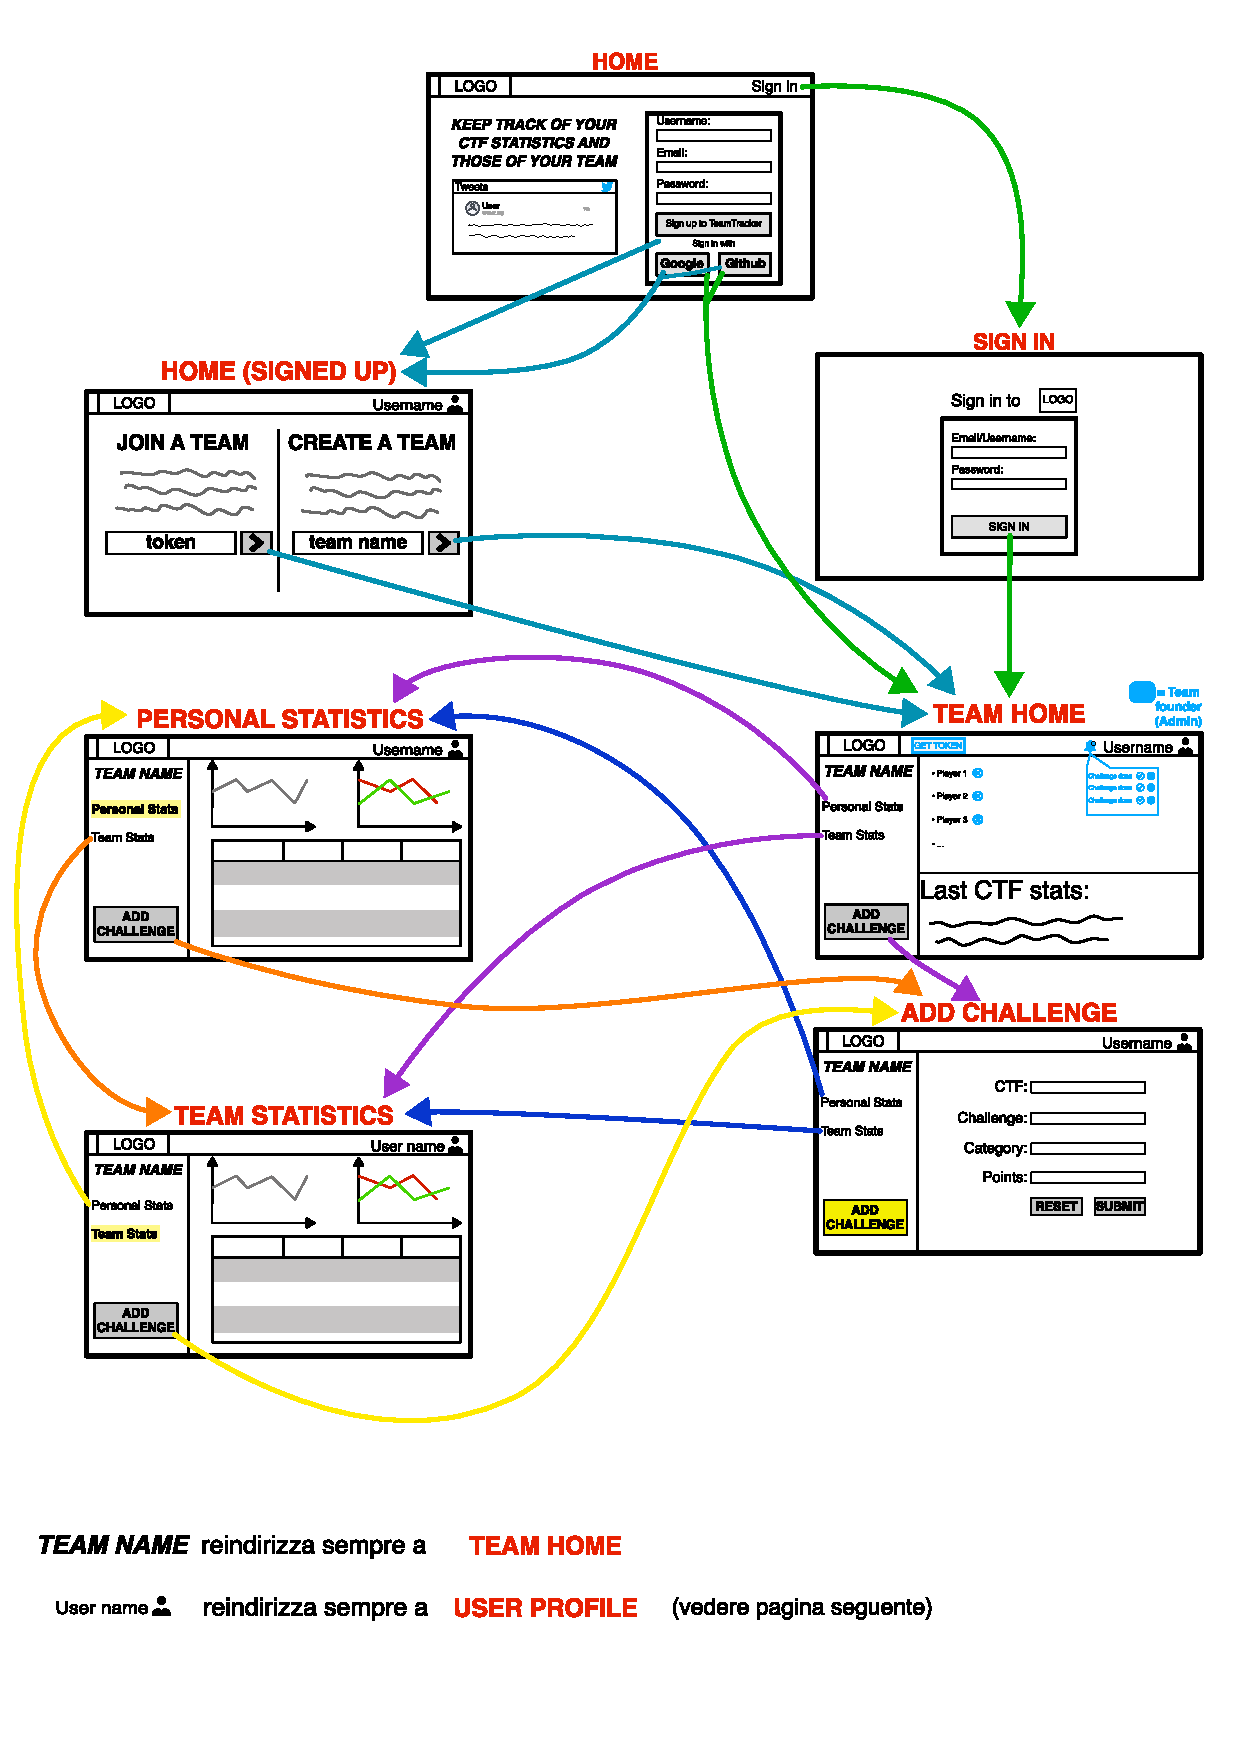
\includepdf[pages=1, scale=0.7, pagecommand=\section{Mockup}]{mockup}
\includepdf[pages=2, scale=0.7]{mockup}

\section{Diagramma E/R}
%\includepdf{er}

\section{Link utili}
\begin{itemize}
    \item Repository Github con codice sorgente: \\ \href{https://github.com/CristianRichie/team-tracker}{https://github.com/CristianRichie/team-tracker}
    \item Tracking degli sprint su Pivotal Tracker: \\ \href{https://www.pivotaltracker.com/n/projects/2327215}{https://www.pivotaltracker.com/n/projects/2327215}
\end{itemize}
\end{document}
